\chapter{Practicum}

\begin{exercise}[Nom nom nom]\mbox{}\\
Bekijk de onderstaande code en beantwoord de volgende vraag zonder de code uit te voeren op je computer:
\begin{enumerate}
    \item Als de node wordt gestart. Welke naam heeft de node dan in ROS?
    % Het antwoord op de onderstaande vraag is wat ingewikkelder dan ik dacht en er blijken meerdere oplossing ervoor zijn mogelijk. Daarom de vraag weg gehaald.
    %\item De main start nu \'e\'en \textit{VoedselNode}. Is het ook mogelijk om twee \textit{VoedselNode}'s te starten in ROS? 
        %\begin{itemize}
        %    \item Zo nee, wat moeten we aanpassen aan de code om dat wel mogelijk te maken?
        %    \item Zo ja, aan welke eisen voldoet de node waardoor dit mogelijk is?
        %\end{itemize}
\end{enumerate}


\begin{minipage}{0.9\linewidth}
\begin{lstlisting}[language=C++, firstnumber=0]
#include "rclcpp/rclcpp.hpp"

class VoedselNode : public rclcpp::Node
{
public:
    VoedselNode();
};

\end{lstlisting}
\end{minipage}

\begin{minipage}{0.9\linewidth}
\begin{lstlisting}[language=C++, firstnumber=0]
#include "rclcpp/rclcpp.hpp"
#include "VoedeselNode.h"

HelloNode::VoedselNode() : Node("Appelkoek"){
    RCLCPP_INFO(this->get_logger(), "Hallo, ik ben Voedsel!");
}
\end{lstlisting}
\end{minipage}

\begin{minipage}{0.9\linewidth}
\begin{lstlisting}[language=C++, firstnumber=0]
#include "rclcpp/rclcpp.hpp"
#include "VoedselNode.hpp"

int main(int argc, char **argv){
    rclcpp::init(argc, argv);
    auto node = std::make_shared<VoedselNode>();
    rclcpp::spin(node); 
    rclcpp::shutdown(); 
    return 0;
}
\end{lstlisting}
\end{minipage}
% antwoorden:
% 1. "appelkoek"
% 2. De constructor van VoedselNode moet een string meekrijgen die we vervolgens meegeven aan 
\end{exercise}

\newpage

\begin{exercise}[Constructieve communicatie]\mbox{}\\
Bekijk de onderstaande code en beantwoord de volgende vragen zonder de code uit te voeren op je computer:
\begin{enumerate}
\item Wat doet de functie \textbf{std::bind()}?
\item Waarom hebben \textit{using std::placeholders::\_1;} nodig?
\item Als we ArchitectNode en BuilderNode (op volgende pagina) runnen wat zien we dan in de terminal verschijnen?
\item ArchitectNode deelt nu drie designs en wacht na het geven van een design even. We willen dat de node tussen elk design 10 seconden wacht. Welke regel moet worden aangepast en wat is de aanpassing?
\item De nodes maken gebruikt van een custom message. Schrijf de custom message.
\end{enumerate}

\begin{minipage}{0.9\linewidth}
\begin{lstlisting}[language=C++, firstnumber=0]
#include "rclcpp/rclcpp.hpp"
#include "ArchitectNode.h"

ArchitectNode::ArchitectNode(): Node("Djoser"){
    publisher_ = this->create_publisher<nijl::msg::design>("designs", 10);

    rclcpp::Rate timer(0.5);
    shareDesign("*", 3);
    timer.sleep();
    shareDesign("#", 7);
    timer.sleep();
    shareDesign("+", 5);
}

void ArchitectNode::shareDesign(std::string pattern, unsigned int n){
  auto message = nijl::msg::design();
  message.pattern = pattern;
  message.n = n;
  publisher_->publish(message);
}
\end{lstlisting}
\end{minipage}

\begin{minipage}{0.9\linewidth}
\begin{lstlisting}[language=C++, firstnumber=0]
#include "rclcpp/rclcpp.hpp"
#include "BuilderNode.h"
#include <string>

using std::placeholders::_1;

BuilderNode::BuilderNode(): Node("Pat en Mat"){
  subscription_ = this->create_subscription<nijl::msg::design>(
    "designs", 10, std::bind(&BuilderNode::designReceiver, this, _1));
}

void BuilderNode::topic_callback(const Nijl::msg::Design::SharedPtr msg) const
{
  unsigned int n = msg->n;
  std::string floor = "";
  for(unsigned int i=0; i < n; i++){
    floor = "";
    for(unsigned int j=0; j < i; j++){
        floor += msg->pattern;
    }
    RCLCPP_INFO(this->get_logger(), floor.c_str());
  }
  for(unsigned int i=n-1; i >= 0; i--){
    floor = "";
    for(unsigned int j=0; j < i; j++){
        floor += msg->pattern;
    }
    RCLCPP_INFO(this->get_logger(), floor.c_str());
  }
}
\end{lstlisting}
\end{minipage}
 % De bedoeling was  een "driehoek"/"pyramide" van sterretjes van 3 hoog dan van #'s 7 hoog en dan van plusjes 5 hoog, echter niet goed gerealiseerd dat RCLCPP_INFO ook een newline neerzet. Resultaat is dus een hele reeks sterretjes, dan een hele reeks #'s en dan een reeks plusjes.
 % de rclcpp::rate timer moet naar 0.1
 % String \n Int64
 % 
\end{exercise}
% YYYYYYYYYYYYYYYYYYYYYYY
% NEWPAGE!!!!!!!!!!!!!
\newpage
% YYYYYYYYYYYYYYYYYYYYYYY
% NEWPAGE!!!!!!!!!!!!!

\begin{exercise}[Interne conversatie]\mbox{}\\
Bekijk de onderstaande code en beantwoord de volgende vragen zonder de code uit te voeren op je computer:
\begin{enumerate}
\item Wat staat er na het starten van de WeirdNode op het scherm?
%Wat heb je?
%Wat heb je
%Wat heb j
%Wat heb 
%Wat heb
%Wat h
%etc.
\item Wat gebeurd er als we twee WeirdNodes starten?
%afhankelijk van timing, waarschijnlijk:%
%%Wat heb je?
%%Wat heb je?
%Wat heb je (4 keer)
%Wat heb j (8 keer)
%Wat heb (16 keer)
%etc.

\end{enumerate}

\begin{minipage}{0.9\linewidth}
\begin{lstlisting}[language=C++, firstnumber=0]
#include "rclcpp/rclcpp.hpp"
#include "std_msgs/msg/string.hpp"
#include "WeirdNode.h"

using std::placeholders::_1; 

WeirdNode::WeirdNode(const std::string & name): Node(name){
    publisher_ = this->create_publisher<std_msgs::msg::String>("topic", 10);

    subscription_ = this->create_subscription<std_msgs::msg::String>(
    "topic", 10, std::bind(&WeirdNode::topic_callback, this, _1));

    std::string content = "Wat heb je?";
    publishMessage(content);
}

void WeirdNode::topic_callback(const std_msgs::msg::String::SharedPtr msg) const {
    std::string content = msg->data.c_str();
    RCLCPP_INFO(this->get_logger(), "I heard: '%s'", content.c_str());

    if(content.size() > 1){:
        std::string new_content = content.substr(0, content.size()-1);
    
        for(int i=0; i<1000000000; i++){} // wait a bit.

        publishMessage(new_content);
    }
}

void WeirdNode::publishMessage(std::string content) const{
    auto message = std_msgs::msg::String();
    message.data = content;
    publisher_->publish(message);
}
\end{lstlisting}
\end{minipage}

\begin{minipage}{0.9\linewidth}
\begin{lstlisting}[language=C++, firstnumber=0]
#include "rclcpp/rclcpp.hpp"
#include "WeirdNode.h"

int main(int argc, char * argv[])
{
  rclcpp::init(argc, argv);
  rclcpp::spin(std::make_shared<WeirdNode>("Weirdo"));
  rclcpp::shutdown();
  return 0;
}
\end{lstlisting}
\end{minipage}

\end{exercise}

\newpage %!!!!!!!!!!!!!newpage!!!!!!!!!!!!!

\begin{exercise}[Abacus]\mbox{}\\
\begin{minipage}{0.6\textwidth}
Maak een package met twee ROS nodes: één publisher en één subscriber. De publisher schrijft elke 2 seconden een willekeurig cijfer op een topic. De subscriber ontvangt drie berichten van het topic en telt deze bij elkaar op. Het resultaat print de subscriber via de logger. De subscriber print dus elke 6 seconden een resultaat. Als de subscriber later start dan de publisher, dan begint de subscriber bij het eerste bericht dat hij ontvangt via het topic (dit is het standaard gedrag van een subscriber).

Zorg er voor dat je package voldoet aan de conventies van ROS2.
\end{minipage}\hfill 
\begin{minipage}{0.3\textwidth}
\begin{center}
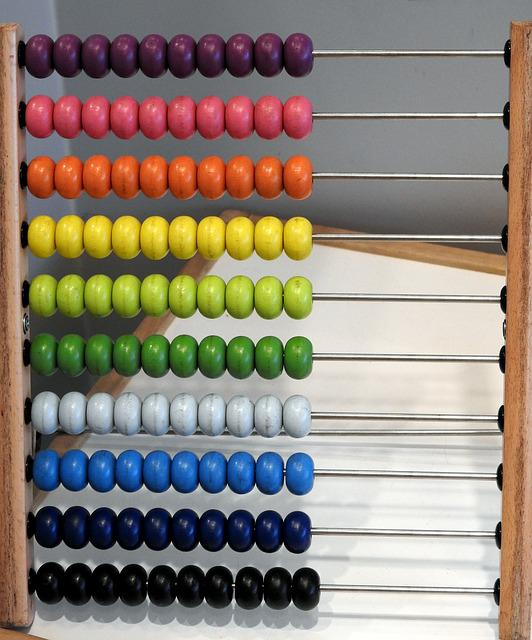
\includegraphics[width=\textwidth]{Pictures/cc_pixabay_abacus.jpg}\\
Een Abacus (ook wel bekend als telraam).\\
\end{center}
\end{minipage}
\end{exercise}

\begin{exercise}[Up and Down]\mbox{}\\
Maak een copy van de package van de opdracht Abacus en gebruik dit als basis voor de opdrachten A en B. 
\subsubsection{A:} 
Pas de publisher aan zodat hij nu willekeurig het woord “plus”, “min” of “keer” stuurt samen met het willekeurige getal. Voorbeeld van berichten op de topic:


\begin{minipage}{0.9\linewidth}
\begin{lstlisting}[style=DOS, firstnumber=0]
plus 8 
min 9 
plus 3 
plus 0 
plus 2 
keer 3
\end{lstlisting}
\end{minipage}

\subsubsection{B:}
Pas ook de subscriber aan, zodat hij de nieuwe berichten van de publisher kan verwerken. Ontvangt de subscriber een bericht met het woord “plus” dan verwerkt hij het getal met een plus. Ontvangt de subscriber een bericht het woord “min” verwerkt hij het getal met een min. Ontvangt de subscriber een bericht het woord “keer” verwerkt hij het getal met een keer. Als het eerste cijfer met het woord “keer” komt, dan verwerkt hij dat als 0 * <getal>.
\end{exercise}

\newpage %!!!!!newpage!!!!!!!

\begin{exercise}[Libellebil]\mbox{}\\
Bekijk onder staande code en beantwoord de onderstaande vragen zonder de code uit te voeren.

\begin{enumerate}
    \item Wat is de service die serviceNode verleend?
    %het draait de string om%
    \item Maak het .srv bestand dat wordt gebruikt door serviceNode.
    %zie codevoorbeelden%
\end{enumerate}

\begin{minipage}{0.9\linewidth}
\begin{lstlisting}[language=C++, firstnumber=0]
#include "rclcpp/rclcpp.hpp"
#include "ServiceNode.h"

using std::placeholders::_1;
using std::placeholders::_2;

ServiceNode::ServiceNode(): Node("ServiceNode"){
    service_ = this->create_service<srvcli_libellebil::srv::Word>(
            "words", 
            std::bind(&ServiceNode::handleService, this, _1, _2)
    );
}

std::string ServiceNode::esrever(std::string word){
    for(size_t i=0; i<word.size()/2; i++){    
        std::swap(word[i], word[word.size()-i-1]);
    }
    return word;
}

void ServiceNode::handleService( 
    const std::shared_ptr<srvcli_libellebil::srv::Word::Request> request,
    std::shared_ptr<srvcli_libellebil::srv::Word::Response> response
){
  std::string outputWord = esrever(request->input_word);

  bool isIt = outputWord == request->input_word;

  response->output_word = outputWord;
  response->is_it = isIt;
}
\end{lstlisting}
\end{minipage}


\end{exercise}

\begin{exercise}[Wijzerplaat]\mbox{}
\begin{minipage}{0.5\textwidth}
\begin{enumerate}
    \item Maak een ROS2 node die functioneert als een analoge klok. De node publiceert de huidige stand van de wijzers eens per seconde.
    \item Maak van de analoge klok node ook een service server. Door middel van de service kan men de klok stopzetten en weer starten.
\end{enumerate}.
\end{minipage}\hfill 
\begin{minipage}{0.4\textwidth}
\begin{center}
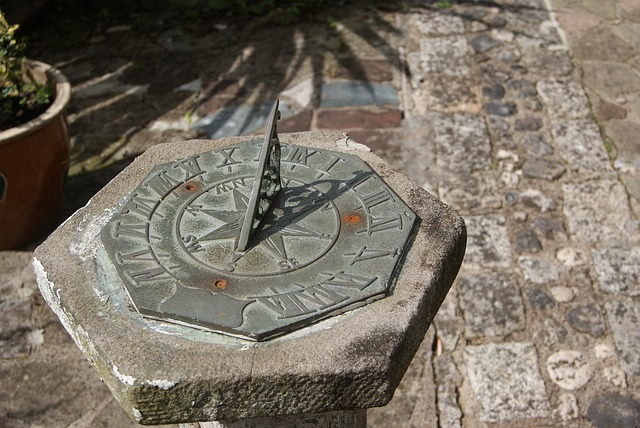
\includegraphics[width=0.95\textwidth]{Pictures/cc_pixabay_zonnwijzer.jpg}\\
Een zonnewijzer.\\
{\tiny(Afbeelding van Mark Caldicott via \url{pixabay.com})}
\end{center}
\end{minipage}
\end{exercise}

\newpage %!!!!!!!!!!!!!!!!newpage!!!!!!!!!

\begin{exercise}[Actie]\mbox{}%Lukt mij niet op een (leuke) zinnige leesopdracht te maken. Daarom maar toevlucht gezocht naar theorievragen. Een suggesties voor een code-leesopdracht over een action-node is welkom.
\begin{enumerate}
    \item Welke berichten bij een action server/client moet je zelf definiëren in de Action message structure?
    \item Welke berichten zijn al voorgedefinieerd bij een action server/client?
\end{enumerate}
\end{exercise}

\begin{exercise}[Conway’s action]\mbox{}\\
Schrijf een ROS action server die de rij van Conway kan bepalen. De rij van Conway staat ook wel bekend als de Look-and-say sequence, omdat het volgende element in de rij wordt gevormd door het huidige element te beschrijven. Meer informatie over de Look-and-say-sequence kan men vinden op:
\begin{itemize}
    \item \url{https://nl.wikipedia.org/wiki/Rij_van_Conway}
    \item \url{https://www.youtube.com/watch?v=ea7lJkEhytA}
\end{itemize}

De action server krijgt als goal de integers \textit{x} en \textit{n} mee. Aan de hand hiervan moet de node de rij van Conway bepalen die begint met \textit{x} en die \textit{n} lang is. De action server geeft elk tussenresultaat terug als feedback naar de action client. Voorbeelden van input van de service en de output staan in de tabel hieronder. Je mag aannemen dat \textit{x} en \textit{n} altijd positief zijn.

\vspace{0.5cm}

\begin{minipage}{0.6\textwidth}

\begin{tabular}{|l|l|p{6cm}|} \hline
\textbf{x} & \textbf{n} & \textbf{Output}  \\ \hline
5 & 3 & 15, 1115, 3115 \\ \hline
367 & 5 & 131617, 111311161117, 311331163117, 1321232116132117, 1113121112131221161113122117  \\ \hline
1 & 7 & 11, 21, 1211, 111221, 312211, 13112221, 1113213211 \\ \hline
9 & 4 & 19 , 1119, 3119, 132119 \\ \hline
\end{tabular}

\end{minipage}\hfill 
\begin{minipage}{0.3\textwidth}
\begin{center}
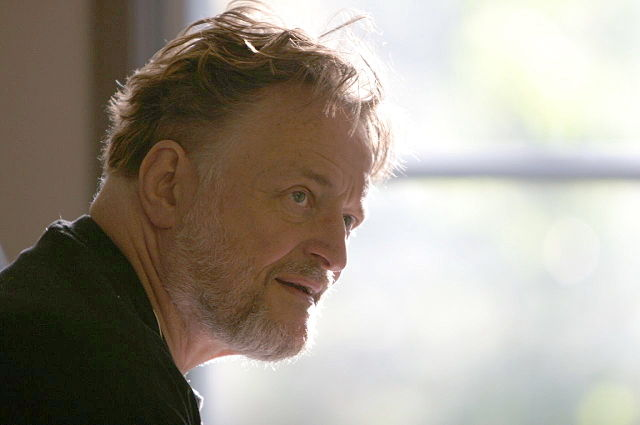
\includegraphics[width=\textwidth]{Pictures/640px-John_H_Conway_2005.jpg}\\
De wiskundige John Conway (1937 - 2020).\\{\tiny(foto door: Thane Plambeck.) \\ \href{https://creativecommons.org/licenses/by/2.0/deed.en}{[CC-BY 2.0]}}\\
\end{center}
\end{minipage}


\vspace{1cm}
\noindent Schrijf ook een action client te testen ook een service client en zorg dat de package voldoet aan de ROS2 conventies. \\

% lukt het de student niet om de het algoritme van conways service te implementeren. Geef deze dan of laat de student een andere service maken. Leerdoel is om een ros2 service te maken.
\end{exercise}

\begin{exercise}[Pijpleiding]\mbox{}\\
Koppel de nodes gemaakt in opdracht 7.5, 7.7 en 7.9 aan elkaar. Bedenk zelf welke nodes met elkaar communiceren. Het kan zijn dat de eerder geschreven nodes een extra of andere communicatierol krijgen en je dus zaken aan je code moet toevoegen.
\end{exercise}